\documentclass[a4paper, 12pt]{article}
\usepackage[utf8]{inputenc}
% \usepackage{fontspec}
\usepackage{hyperref}
\usepackage{graphicx}
\usepackage{changepage}
\graphicspath{ {images/} }
\usepackage[a4paper,left=1.5in,right=1in,top=1in,bottom=1in]{geometry}
\usepackage{times}
\usepackage{epsfig}
\usepackage{tikz}
\usetikzlibrary{positioning,shapes,fit,arrows}
\definecolor{myblue}{RGB}{56,94,141}
\usepackage{fancyhdr}
\usepackage{booktabs}
\usepackage{mathtools}
\usepackage{amsmath}
\usepackage{amssymb}
\usepackage{enumitem}
\usepackage{etoolbox}
%\apptocmd{\thebibliography}{\csname phantomsection \endcsname \addtocontentsline{toc}{chapter}{\bibname}}{}{}
\usepackage{caption}
\usepackage{float}
\floatstyle{boxed} 
\restylefloat{figure}
\pagestyle{fancy}
\fancyhf{}
% \fancyhead[LE,RO]{\footnotesize \center }
% \fancyfoot[CE,CO]{ \raggedright{\fontfamily{cmr}\select P:F-SMR-UG/08/R0}}
\fancyfoot[LE,RO]{\thepage}
\def\eg{\textit{e.g.}~}
\def\ie{\textit{i.e.}~}
\def\Eg{\textit{E.g.}~}
\def\etal{\textit{et al.}~}
\def\etc{\textit{etc.}~}
\def\ci#1{\textcircled{\resizebox{.4em}{!}{#1}}}
\renewcommand{\baselinestretch}{1}

\newcommand{\thr}[1]{\rotatebox[origin=c]{90}{#1}}
\newcommand{\tht}[2]{\begin{tabular}{@{}#1@{}}#2\end{tabular}}
\newcommand{\red}[1]{\textcolor{blue}{#1}}
\usepackage{hyperref}
\hypersetup{
    colorlinks=true,
    linkcolor=blue,
    filecolor=magenta,      
    urlcolor=cyan,
}
% \setsansfont{arial.ttf}
\usepackage[nottoc]{tocbibind} %Adds "References" to the table of contents

\begin{document}
 
\begin{titlepage}
    \begin{center}
        \vspace*{1cm}
        
        \large
                \textbf{\MakeUppercase{Pune Institute of Computer Technology}}
                \linebreak
        \textbf{\MakeUppercase{Dhankawadi, Pune}}
        \vspace{0.5cm}
                        \linebreak
                        \linebreak
        \MakeUppercase{High Performance Computing Mini-Project REPORT }
        \linebreak
        ON
        \linebreak
        \vspace{0.5cm}
        \large
        \\
        \textbf{\MakeUppercase{“Generic Compression - Run length encoding
concurrently on multi$-$core. ”}}
        \linebreak
        
        %\vspace{0.2cm}
        \textbf{SUBMITTED BY}
        \vspace{1cm}
        
        \begin{center}
        \begin{tabular}{ c c }
         Nachiket Erlekar & 41434 \\ 
         Ashay Koradia & 41429 
        \end{tabular}
        \end{center}
                
        \textbf{\large{Under the guidance of}}
        \linebreak
        Prof. Deepali Kadam
        \linebreak
      %  \vfill
        
        
        
        \vspace{0.8cm}
        

        
\includegraphics[scale=0.6]{pict.eps}   
        
        \Large
        DEPARTMENT OF COMPUTER ENGINEERING\\
%        \textbf{Pune Institute of Computer Technology}    
%        \textbf{Dhankawadi, Pune}
%        \linebreak
        \textbf{Academic Year 2020-21}
        
    \end{center}
\end{titlepage}
\pagebreak

\newpage
\tableofcontents

\newpage
\pagenumbering{arabic}
\begin{center}
    \section{Problem Statement}
\end{center}

Perform Run length encoding concurrently on many core GPU. Run-length encoding is a form of lossless data compression in which runs of data (sequences in which the same data value occurs in many consecutive data elements) are stored as a single data value and count, rather than as the original run.

\newpage
\begin{center}
    \section{Abstract}
\end{center}
Multi-core programming is increasingly used for acceleration of data-parallel functions, such as
image transforms and motion estimation. However, the entropy coding stage is typically executed
on the CPU due to inherent data dependencies in lossless compression algorithms. We propose a
simple way of efficiently dealing with these dependencies, and present a parallel compression
algorithm specifically designed for efficient execution on many-core architectures. By
parallelization of lossless compression algorithms not only do we significantly speed-up the
entropy coding, but we also enable completion of all encoding phases using OpenMPI.


\newpage
\begin{center}
\section{INTRODUCTION}
\end{center}
\hspace{1cm}
\par

In the Run Length Encoding, we need to compute the indexes of the elements to be stored and their codes i.e. the length of the symbol run. The first approach for computing the codes is based on the use of another parallel primitive, the reduction, for counting the symbol or summing up the number of times a symbol appeared in its run. Further analysis of dependencies in the original algorithm resulted in a method which does not depend on the architectural support for the atomic operations. Instead of summing the number of occurrences for each symbol in parallel, the indexes of last elements in each of the run are determined on the basis of the flags. These index values then can be used to compute the total number of elements that appear in between these locations without actually counting the occurrences. The resulting count corresponds to the number of times an element appeared in its run.



\newpage
\begin{center}
\section{OBJECTIVE}
\end{center}
\begin{itemize}
    \item To implement a generic compression algorithm using parallelism.
    \item To compare the speed-up and efficiency of serial and parallel implementation of
run-length encoding compression algorithm.
\end{itemize}


\newpage
\begin{center}
\section{Scope}
\end{center}

This parallel compression algorithm can be easily combined with the already available GPU-accelerated
image transforms and motion estimation algorithms, to enable execution of all codec components directly
on GPUs. With this approach we speed-up the entropy coding by 5-20x, and reduce the data transfer time
from the GPU to system memory.
\newpage
\begin{center}
\section{Test Cases}
\end{center}
\begin{verbatim}
Files :
input1 => average case
input2 => worst case
input3 => best case
    
\end{verbatim}
\begin{center}
    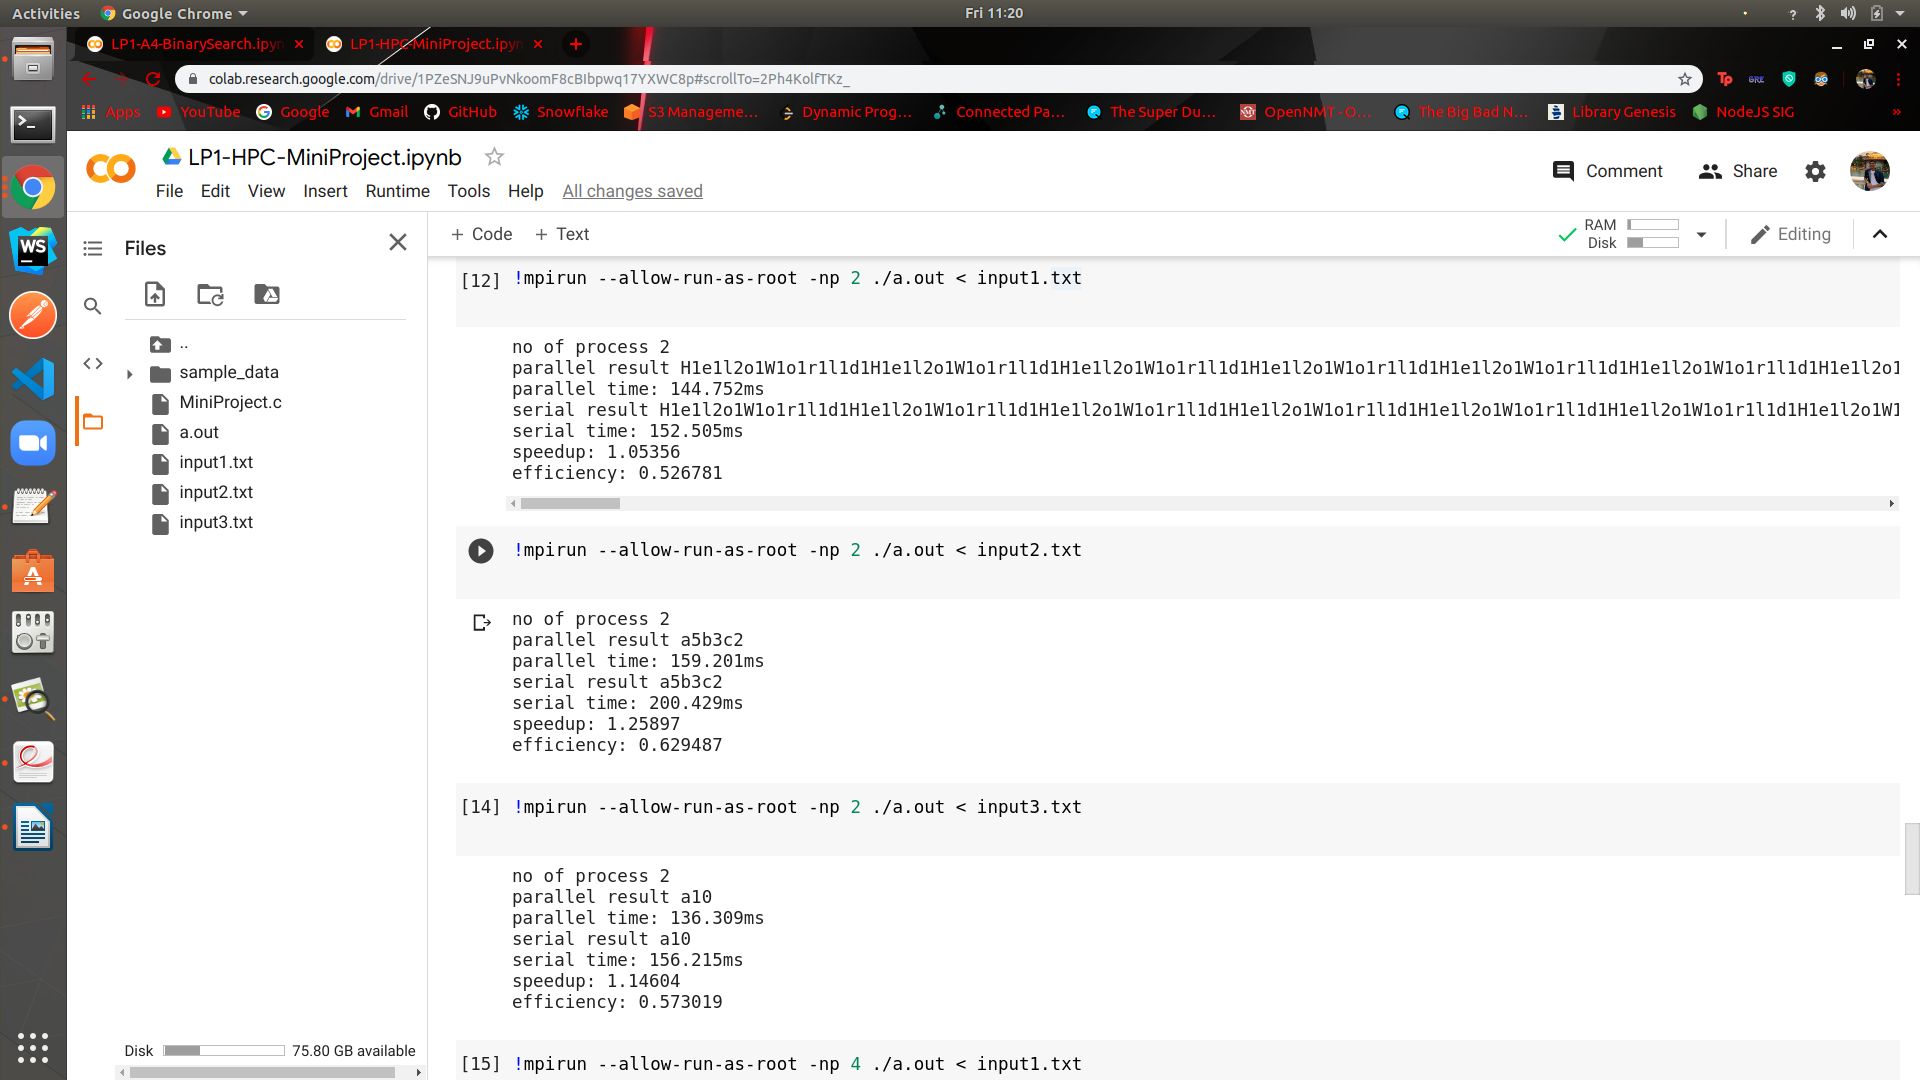
\includegraphics[width=\linewidth]{2_.png}
     \captionof{figure}{Output with no. of processes 2}
\end{center}
\par
\begin{center}
    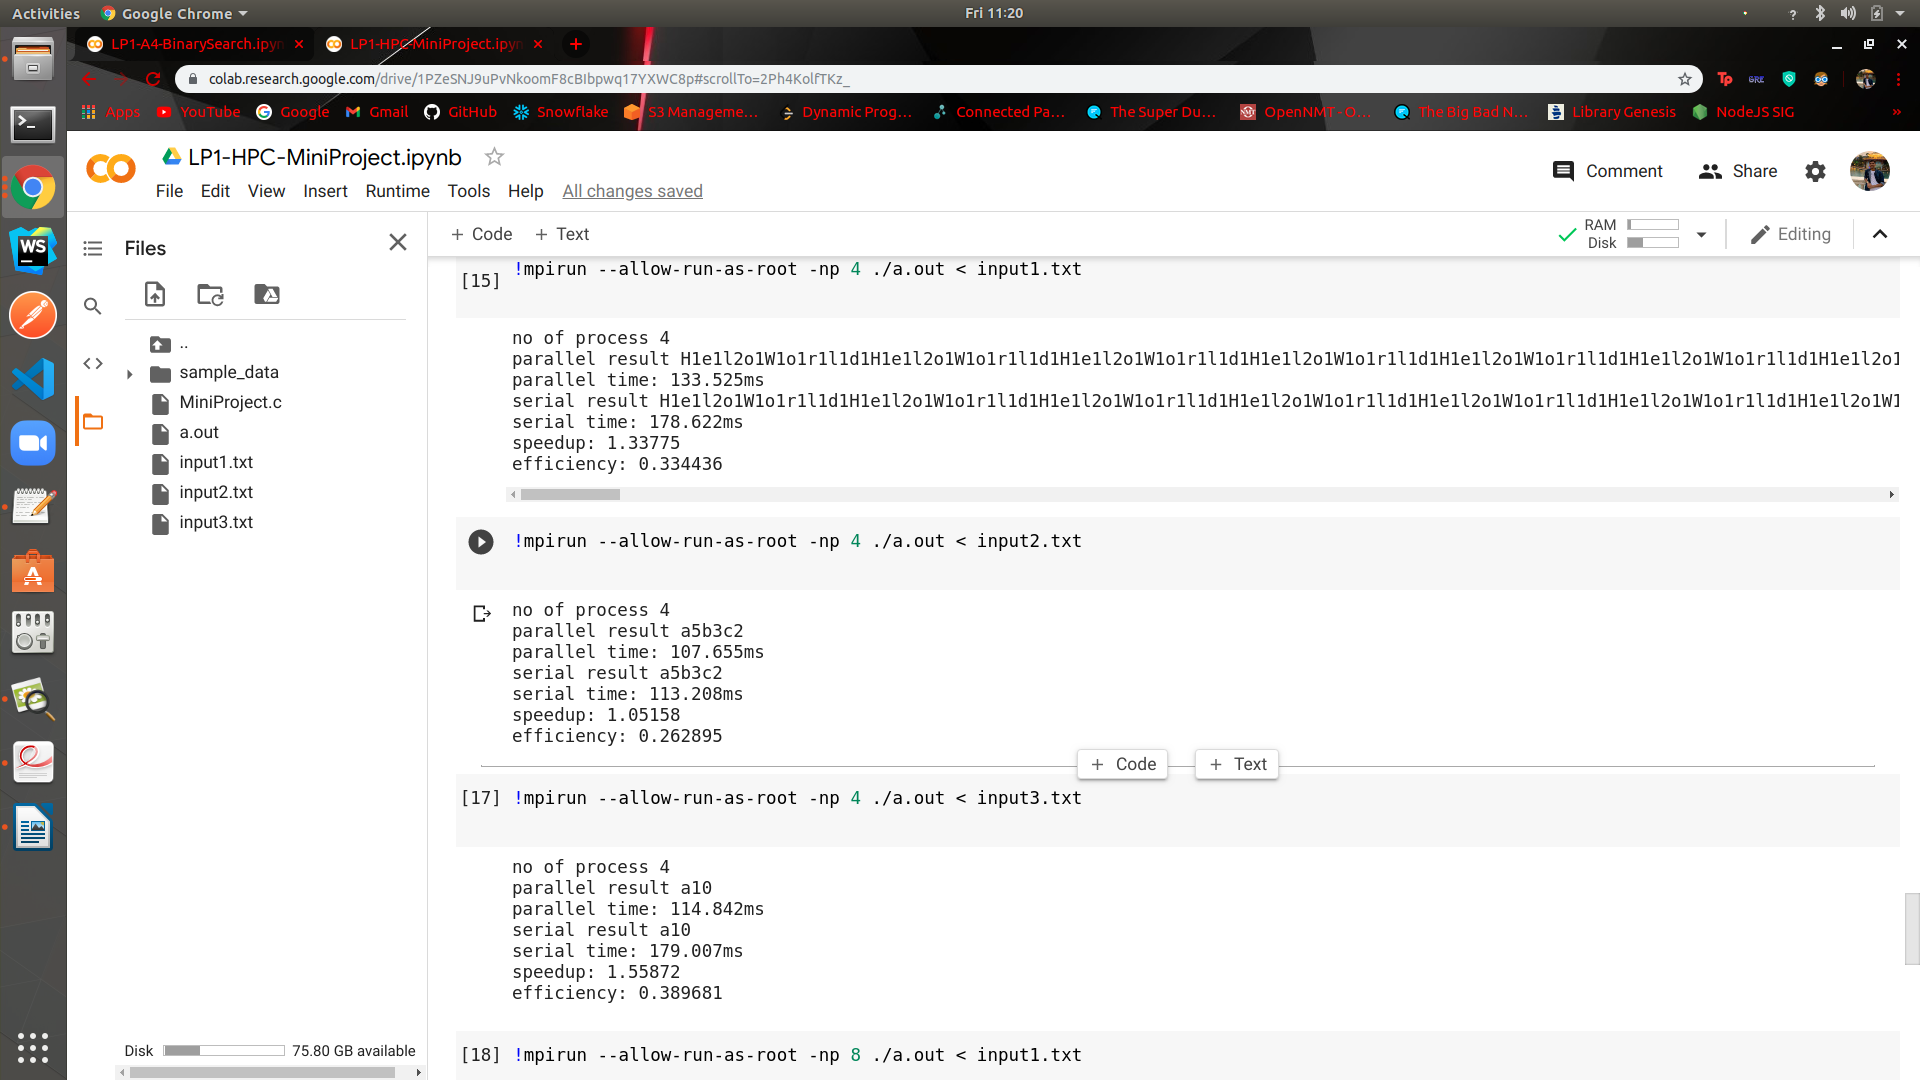
\includegraphics[width=\linewidth]{4_.png}
     \captionof{figure}{Output with no. of processes 4}
\end{center}
\par
\begin{center}
    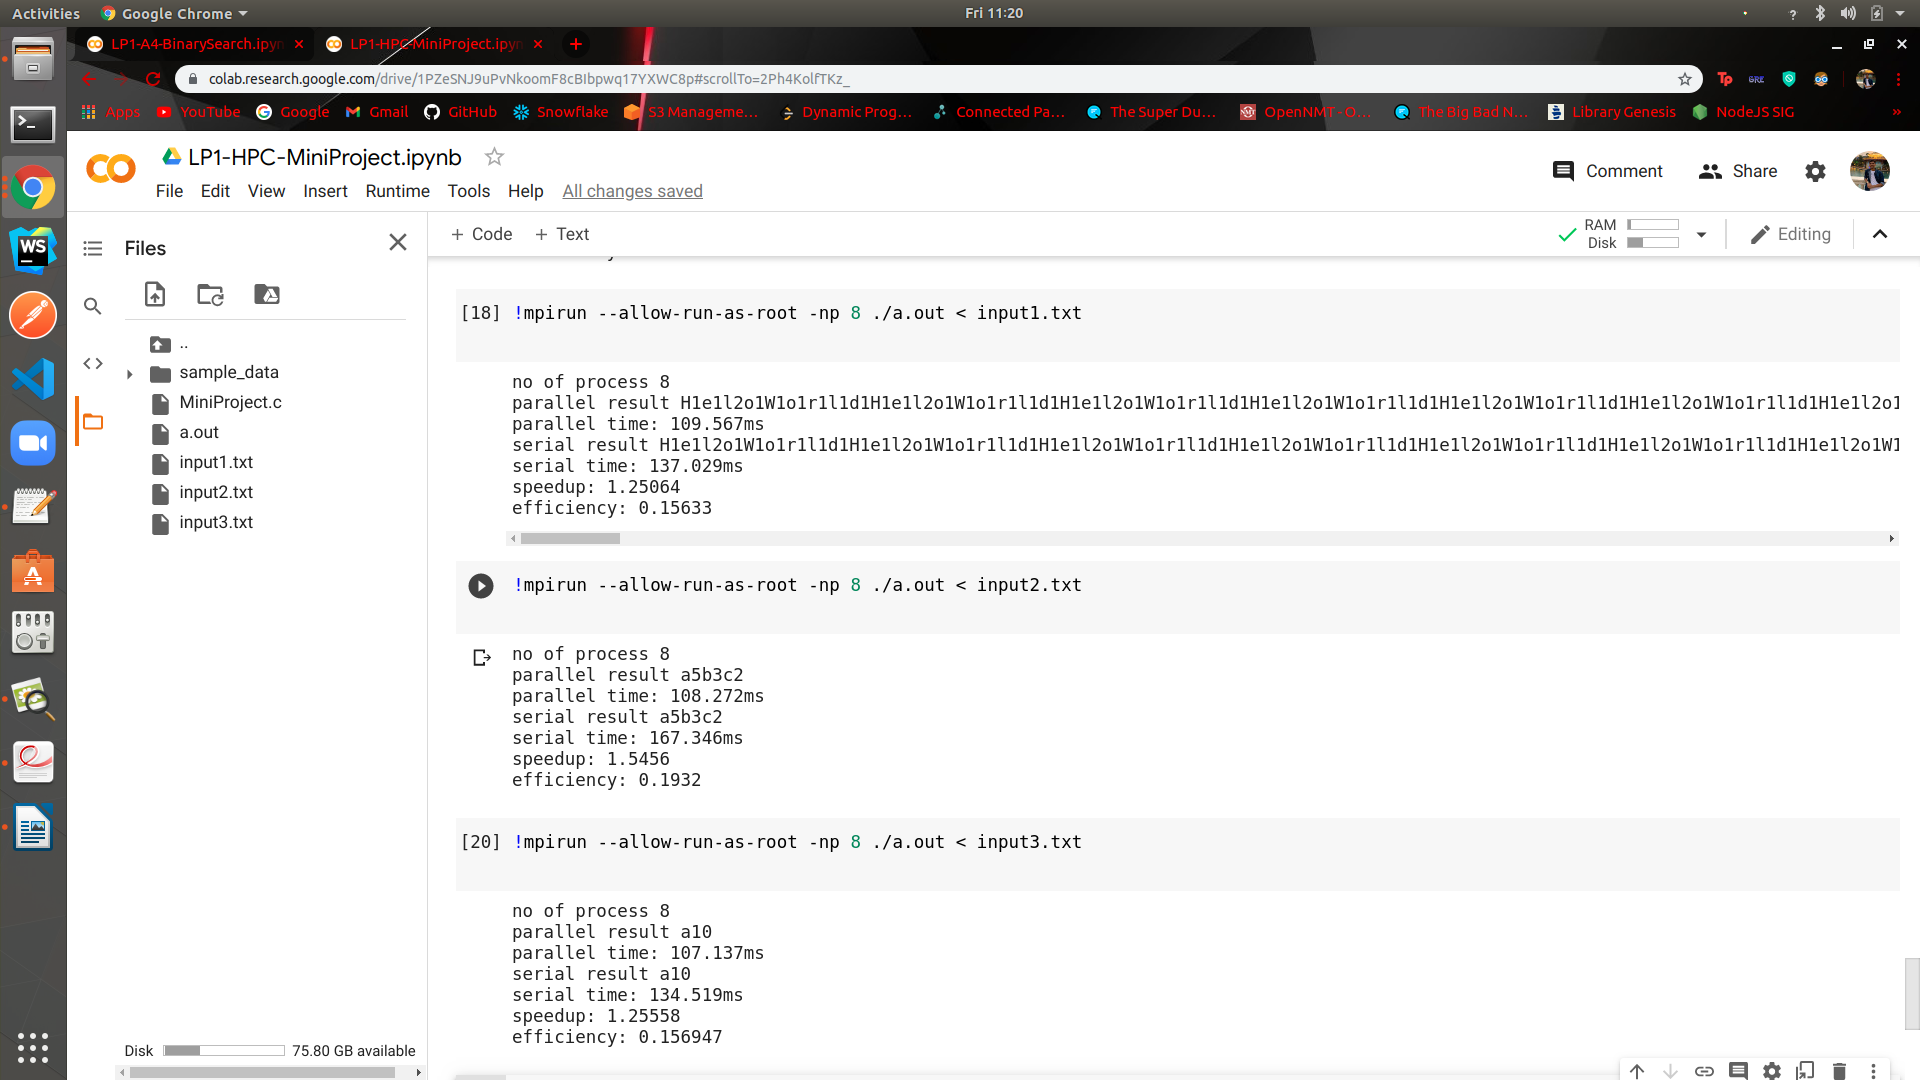
\includegraphics[width=\linewidth]{8_.png}
     \captionof{figure}{Output with no. of processes 8}
\end{center}
\newpage
\begin{center}
\section{Result}
\end{center}
 Highest speedup and efficiency is given when 4 process are used for all i.e best case, worst case and
average case.
\newpage
\begin{center}
\section{Conclusion}
\end{center}
We presented parallel lossless compression designed for efficient execution on many core architectures
supporting parallelism. The parallelization of the Run-Length encoding resulted in processing rates up to
2x speedup.

\newpage
\begin{thebibliography}{1}
\bibitem{gfg}
\texttt{https://www.geeksforgeeks.org/run-length-encoding/}
\bibitem{stackoverflow}
\texttt{https://stackoverflow.com/questions/31890523/how-to-use-mpi-gatherv-for-collecting-strings-of-diiferent-length-from-different}
\bibitem{openmpi}
\texttt{https://www.open-mpi.org/doc/v4.0/}
\end{thebibliography}
\end{document}
